\section{Experiment}
In this section we describe our procedure for testing the efficacy of our feature extraction pipeline and machine learning methods. First we introduce our chosen test bench and metrics, followed by experiment setups.

\begin{figure}[t]
\begin{center}
   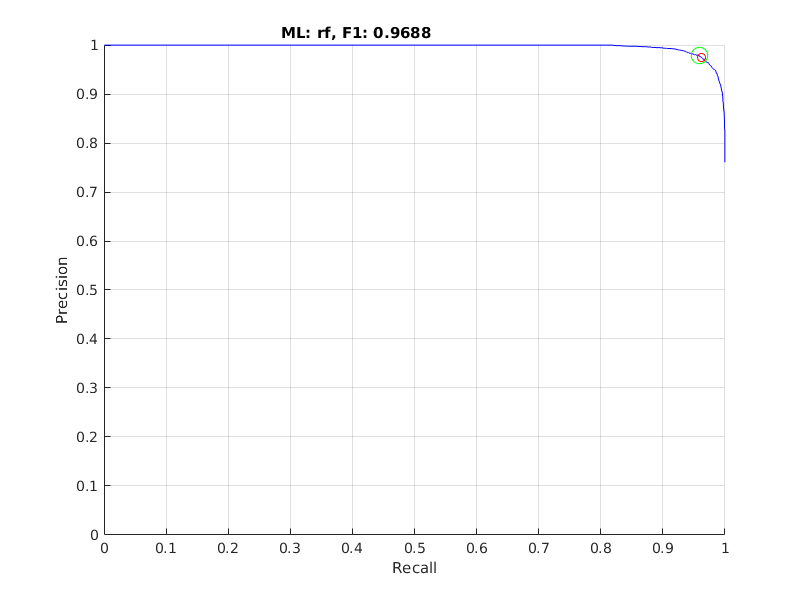
\includegraphics[width=0.8\linewidth]{./figures/siaf.png}
\end{center}
 \vspace{-0.4cm}
   \caption{Performance of the the random forest classifier using same input with all features}
   \vspace{-0.3cm}
\label{fig:siaf}
\end{figure}

\subsection{Test Bench}
We use MiBench \cite{guthaus2001mibench} as our test bench for fault injection. MiBench is a representative embedded benchmark that offers compact program sizes and versatile program characteristics. Specifically, qsort is chosen as our test program.

\subsection{Metrics}
To evaluate the performance of our machine learning method, we use precision-recall (PR) curve and $F_1$ score as our criteria due to unbalanced positive and negative samples. More precisely, we have
\begin{equation}
F_{1} = 2\cdot\frac{precision \cdot recall}{precision + recall},
\end{equation}
where $precision = \frac{tp}{tp+fp}$, $recall = \frac{tp}{tp+fn}$, $tp$ is the number true positive samples, $fp$ is number of false positive samples, and $fn$ is the number of false negative samples. Essentially, $F_1$ score is the harmonic mean of precision and recall. PR curve can reflect the performance of the classifier well since it takes the number of false positives into account, which is prevalent in our testing instances. For identifying fault types, which is a multi-class classification problem, we use confusion matrix to describe the performance of our classifier. Each column of a confusion matrix is the samples in a predicted category whereas each row is the samples in ground truth \cite{powers2011evaluation}.

\subsection{Experiment Setup}
We present four types of experiment setup: 1) same input data (for qsort) with all features, 2) same input data with handpicked subsets of features, 3) different input data with all meaningful features, and 4) different input data with handpicked subsets of features. We would like to examine how different input and sets of feature  may affect the performance of our pipeline in order to explore the optimal setup for detecting faults.

\section{Result}
In this section we report results of all four types of experiment setup. For PR curves, they represent the performance of binary classification (whether the program output is correct) given predictions from random forest. For confusion matrices, they represents the how well our classifier can identify different types of faults.

\begin{figure}[t]
\begin{center}
   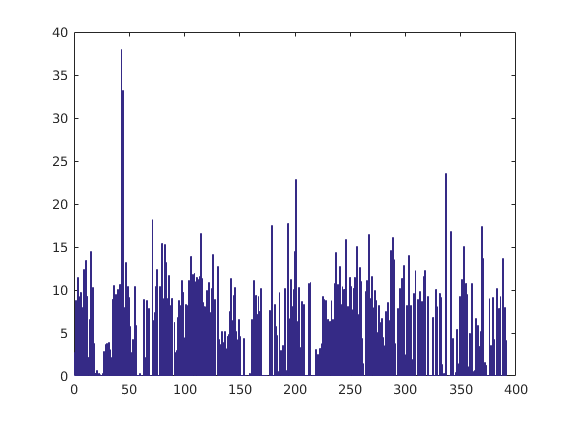
\includegraphics[width=0.8\linewidth]{./figures/feat_same.png}
\end{center}
 \vspace{-0.4cm}
   \caption{Feature importance ranking of SIAF}
   \vspace{-0.3cm}
\label{fig:feat-same}
\end{figure}

\subsection{Same Input All Features (SIAF)}
Figure~\ref{fig:siaf} shows the performance of our binary classifier given all features from stats file and \emph{qsort} uses the same input data. Our approach works well in this task since the $F_1$ score is 0.9688 (max $F_1$ value: 1) and the shape of PR curve is almost perfect (a curve started at $(0,1)$, reached $(1,1)$, and stopped at $(1,0)$). 

We further examine the feature importance ranking extracted from the random forest, as illustrated in Figure~\ref{fig:feat-same}. The y-axis represents information gain and each bar along the x-axis represent one feature dimension. Several features in Figure~\ref{fig:feat-same} shows high discriminative power, which entails that a handful features are able to predict the outcome of the program. The top-3 discriminative features are 
\begin{itemize}
\item $sim\_insts$: \\
Number of instructions simulated
\item $system.cpu.fetch.insts$: \\
Number of instructions fetch has processed
\item $system.cpu.dcache.tags.occ\_percent::cpu.data$: \\
Average percentage of cache occupancy
\end{itemize}


We further extend the capability of our classifier to predict the fault types instead of only determining program outcome.
Figure~\ref{fig:siaf-multi} shows the confusion matrix of \emph{SIAF}. A perfect confusion matrix would be light yellow color appears in the diagonal entries and the rest is dark blue. According to Figure~\ref{fig:siaf-multi}, our classifier can recognize correct program outcome, \emph{general fetch} fault and \emph{load/store} fault quite well. However, it doesn't perform well on \emph{execution} and \emph{opcode} fault. We suspect that this is due to the variances of those two types of faults, and we may need more training data of those two types of faults to train the classifier.

\begin{figure}[ht]
\begin{center}
   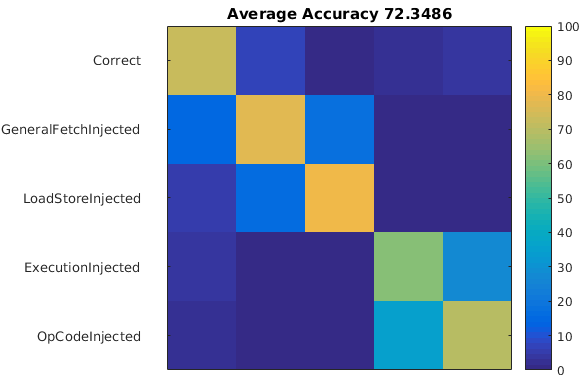
\includegraphics[width=0.8\linewidth]{./figures/siaf_multi.png}
\end{center}
    \vspace{-0.4cm}
   \caption{Fault type classification using SIAF.}

\label{fig:siaf-multi}
\vspace{-0.3cm}
\end{figure}

\subsection{Same Input Different Features}
In order to examine how different sets of features may affect the performance, we further compare the PR curves of different feature sets. The broken line in Figure~\ref{fig:sidf} represents the result of using all features, which clearly outperforms all other handpicked feature. Among handpicked features, the classifier trained using $l2$ cache features performs slightly better than the rest, whereas the classifier trained using decode features performs the worst.

\begin{figure}[t]
\begin{center}
   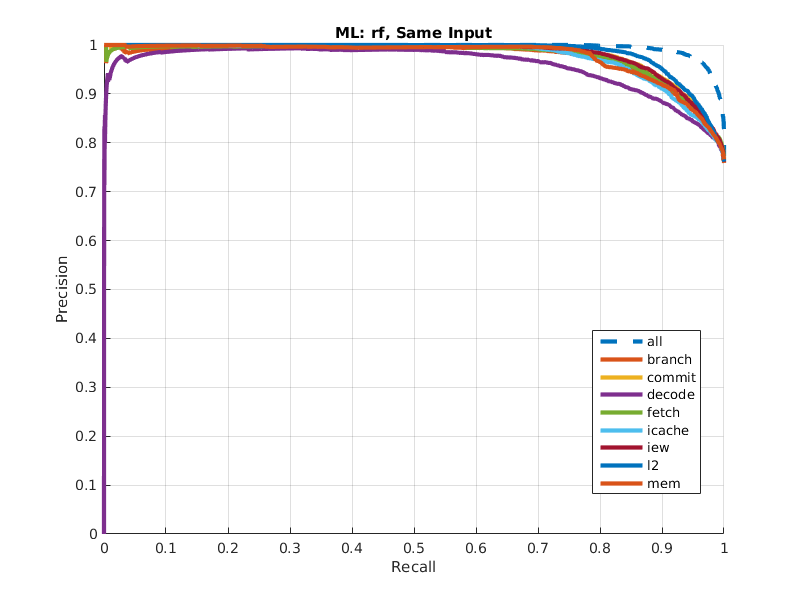
\includegraphics[width=0.95\linewidth]{./figures/sidf.png}
\end{center}
    \vspace{-0.4cm}
   \caption{Comparison among classifiers trained on different sets of features using the same input data.}

\label{fig:sidf}
\vspace{-0.3cm}
\end{figure}

\subsection{Different Input}
All previous results are based on the same input data, which may not be convincing in the real-world situation. Thus, we give \emph{qsort} different input and retrain the random forest classifier.

\begin{figure}[t]
\begin{center}
   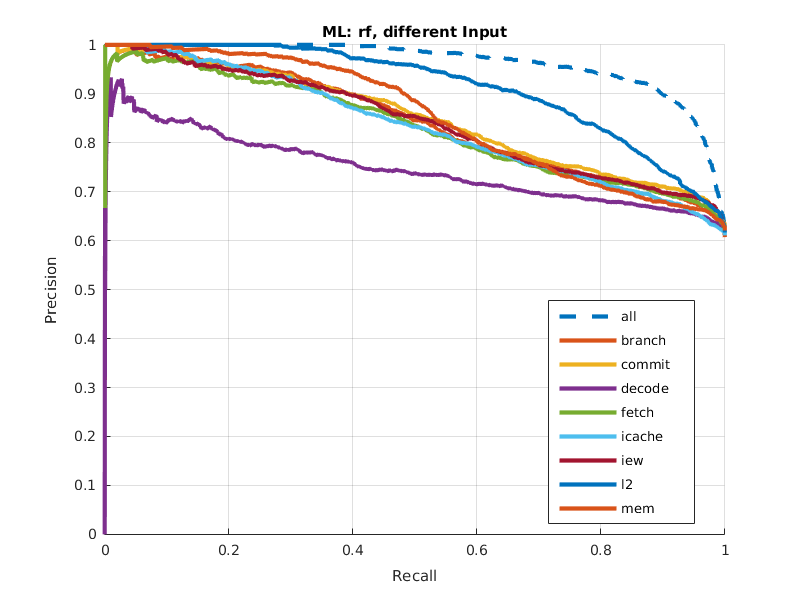
\includegraphics[width=0.8\linewidth]{./figures/didf.png}
\end{center}
    \vspace{-0.4cm}
   \caption{Fault type classification using different input data.}

\label{fig:didf}
\vspace{-0.3cm}
\end{figure}

Figure~\ref{fig:didf} shows the binary classification results using different input data. The broken line represents the classifier with all features, which outperform the all other hand-picked features. This, again, demonstrates that hand-picked features may not outperform the classifier that uses all features.

\begin{figure}[t]
\begin{center}
   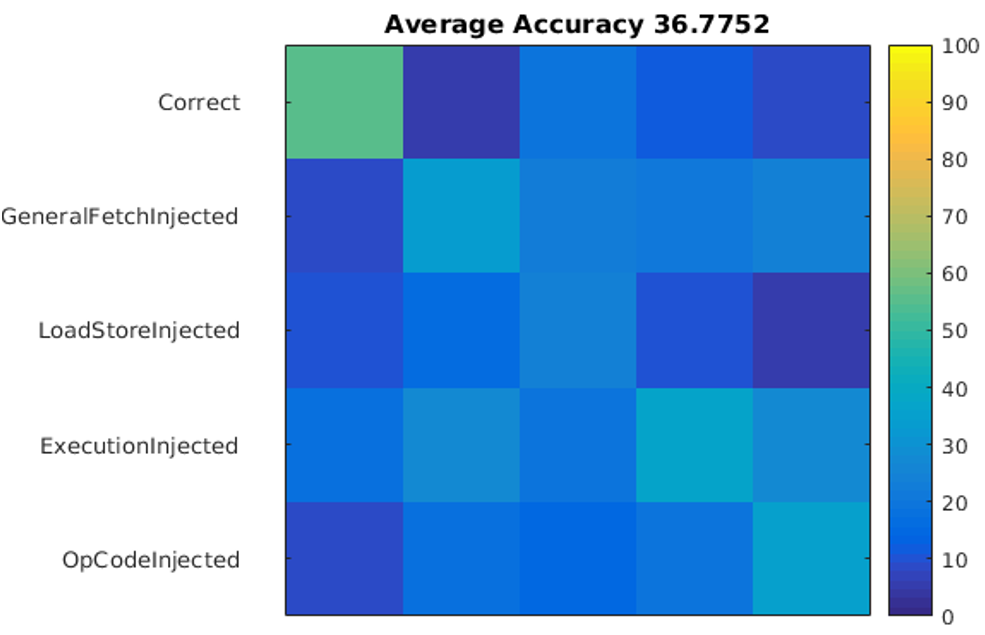
\includegraphics[width=0.8\linewidth]{./figures/diaf_multi.png}
\end{center}
 \vspace{-0.4cm}
   \caption{Comparison among classifiers trained on different sets of features using the different input data.}
\label{fig:diaf-multi}
   \vspace{-0.3cm}
\end{figure}

Figure~\ref{fig:didf} shows the confusion matrix of fault prediction using different input data. Comparing to Figure \ref{fig:siaf-multi}, its performance is much worse. One reason is that different input data bring significant variance into the training data, which would require more training data to sufficiently train a classifier. Thus, given the same amount of training data, the classifier with different input data would unequivocally underperform the one with the same input data.

